\chapter{Derivatives}

\section{Real-valued functions}

\subsection*{Definitions and Theorems}

\begin{definition}[Derivative]
The derivative of a function $f$ at a point $c$ is defined as
\[ f'(c) = \lim_{x \to c} \frac{f(x) - f(c)}{x - c} = \lim_{h \to 0} \frac{f(c + h) - f(c)}{h} \]
if this limit exists.
\end{definition}

\begin{definition}[Differentiable Function]
A function $f$ is differentiable at a point $c$ if $f'(c)$ exists. A function is differentiable on an interval if it is differentiable at every point in that interval.
\end{definition}

\begin{definition}[Lipschitz Condition]
A function $f$ satisfies a Lipschitz condition of order $\alpha$ at $c$ if there exists a positive number $M$ and a neighborhood $B(c)$ of $c$ such that
\[ |f(x) - f(c)| \leq M|x - c|^\alpha \]
whenever $x \in B(c)$.
\end{definition}

\begin{theorem}[Differentiability Implies Continuity]
If a function $f$ is differentiable at a point $c$, then $f$ is continuous at $c$.
\end{theorem}

\begin{theorem}[Basic Differentiation Rules]
For differentiable functions $f$ and $g$:
\begin{enumerate}
\item $(f + g)'(x) = f'(x) + g'(x)$ (sum rule)
\item $(fg)'(x) = f'(x)g(x) + f(x)g'(x)$ (product rule)
\item $\left(\frac{f}{g}\right)'(x) = \frac{f'(x)g(x) - f(x)g'(x)}{g(x)^2}$ (quotient rule)
\item $(f \circ g)'(x) = f'(g(x))g'(x)$ (chain rule)
\end{enumerate}
\end{theorem}

\begin{theorem}[Leibniz's Formula]
For functions $f$ and $g$ with $n$th derivatives, the $n$th derivative of their product is
\[ (fg)^{(n)}(x) = \sum_{k=0}^{n} \binom{n}{k} f^{(k)}(x)g^{(n-k)}(x) \]
\end{theorem}

\begin{theorem}[Schwarzian Derivative]
The Schwarzian derivative of a function $f$ is defined as
\[ Sf(x) = \frac{f'''(x)}{f'(x)} - \frac{3}{2}\left(\frac{f''(x)}{f'(x)}\right)^2 \]
\end{theorem}

\begin{theorem}[Wronskian]
For functions $f_1, \ldots, f_n$ with $(n-1)$th derivatives, the Wronskian is the determinant
\[ W(f_1, \ldots, f_n)(x) = \begin{vmatrix}
f_1(x) & f_2(x) & \cdots & f_n(x) \\
f_1'(x) & f_2'(x) & \cdots & f_n'(x) \\
\vdots & \vdots & \ddots & \vdots \\
f_1^{(n-1)}(x) & f_2^{(n-1)}(x) & \cdots & f_n^{(n-1)}(x)
\end{vmatrix} \]
\end{theorem}

In the following exercises assume, where necessary, a knowledge of the formulas for differentiating the elementary trigonometric, exponential, and logarithmic functions.

\begin{problembox}[5.1: Lipschitz Condition and Continuity]
A function \( f \) is said to satisfy a Lipschitz condition of order \( \alpha \) at \( c \) if there exists a positive number \( M \) (which may depend on \( c \)) and a 1-ball \( B(c) \) such that 
\[ |f(x) - f(c)| < M|x - c|^\alpha \]
whenever \( x \in B(c), x \neq c \).

a) Show that a function which satisfies a Lipschitz condition of order \( \alpha \) is continuous at \( c \) if \( \alpha > 0 \), and has a derivative at \( c \) if \( \alpha > 1 \).

b) Give an example of a function satisfying a Lipschitz condition of order 1 at \( c \) for which \( f'(c) \) does not exist.
\end{problembox}

\noindent\textbf{Strategy:} For (a), use the Lipschitz condition to show that $|f(x) - f(c)| \to 0$ as $x \to c$ when $\alpha > 0$, and that the difference quotient tends to 0 when $\alpha > 1$. For (b), use the absolute value function at $x = 0$ which has a corner and no derivative.

\bigskip\noindent\textbf{Solution:}
If $\alpha>0$ then $|f(x)-f(c)|\le M|x-c|^{\alpha}\to 0$ as $x\to c$, so $f$ is continuous at $c$. If $\alpha>1$ then, for $x\ne c$,
\[\left|\frac{f(x)-f(c)}{x-c}\right|\le M|x-c|^{\alpha-1}\to 0,\]
so $f'(c)=0$ exists. For (b), $f(x)=|x|$ satisfies a Lipschitz condition of order $1$ at $0$, but $f'(0)$ does not exist.\qed


\begin{problembox}[5.2: Monotonicity and Extrema]
In each of the following cases, determine the intervals in which the function \( f \) is increasing or decreasing and find the maxima and minima (if any) in the set where each \( f \) is defined.
a) \( f(x) = x^3 + ax + b, \quad x \in \mathbb{R} \).
b) \( f(x) = \log (x^2 - 9), \quad |x| > 3 \).
c) \( f(x) = x^{2/3}(x - 1)^4, \quad 0 \leq x \leq 1 \).
d) \( f(x) = (\sin x)/x \) if \( x \neq 0, f(0) = 1, \quad 0 \leq x \leq \pi /2 \).
\end{problembox}

\noindent\textbf{Strategy:} For each function, find the derivative and analyze its sign to determine intervals of increase/decrease. For (a), consider the sign of the quadratic derivative. For (b), use the chain rule and analyze the sign. For (c), use logarithmic differentiation. For (d), use the quotient rule and analyze the sign of the derivative.

% Plot for Problem 5.2: Function behavior analysis
\begin{figure}[h]
\centering
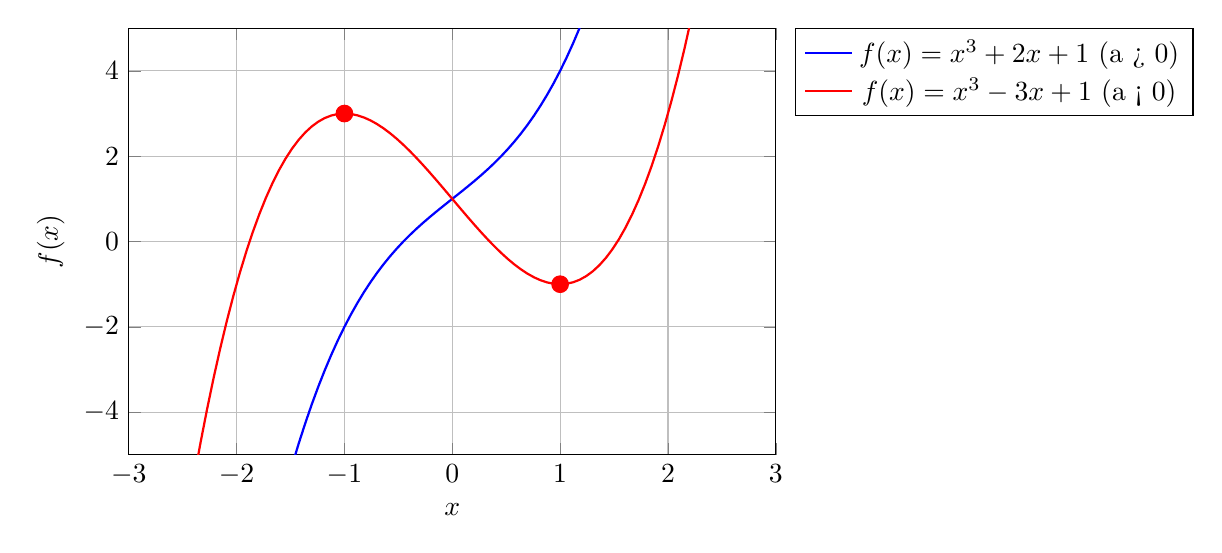
\begin{tikzpicture}
    \begin{axis}[
        width=9.8cm,
        height=7cm,
        xlabel={$x$},
        ylabel={$f(x)$},
        xmin=-3, xmax=3,
        ymin=-5, ymax=5,
        grid=major,
        legend pos=outer north east
    ]
    
    % Plot (a): f(x) = x^3 + ax + b with different a values
    \addplot[blue, thick, samples=100, domain=-3:3] {x^3 + 2*x + 1};
    \addlegendentry{$f(x) = x^3 + 2x + 1$ (a > 0)}
    
    \addplot[red, thick, samples=100, domain=-3:3] {x^3 - 3*x + 1};
    \addlegendentry{$f(x) = x^3 - 3x + 1$ (a < 0)}
    
    % Mark critical points for a < 0 case
    \addplot[only marks, mark=*, mark size=3pt, red] coordinates {
        (-1, 3) (1, -1)
    };
    
    \end{axis}
\end{tikzpicture}
\caption{Problem 5.2: Function behavior analysis showing cubic functions with different parameter values. The blue curve shows a strictly increasing function (a > 0), while the red curve shows a function with local extrema (a < 0).}
\end{figure}

\begin{figure}[h]
\centering
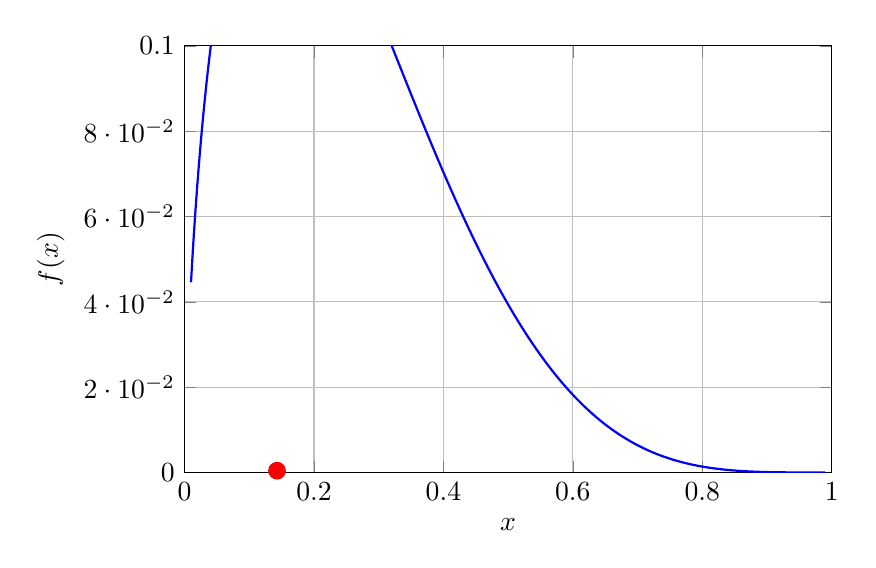
\begin{tikzpicture}
    \begin{axis}[
        width=9.8cm,
        height=7cm,
        xlabel={$x$},
        ylabel={$f(x)$},
        xmin=0, xmax=1,
        ymin=0, ymax=0.1,
        grid=major
    ]
    
    % Plot (c): f(x) = x^(2/3)(x-1)^4
    \addplot[blue, thick, samples=1000, domain=0.01:0.99] {x^(2/3) * (x-1)^4};
    
    % Mark the maximum point
    \addplot[only marks, mark=*, mark size=3pt, red] coordinates {
        (0.142857, 0.000416)
    };
    
    \end{axis}
\end{tikzpicture}
\caption{Problem 5.2(c): The function $f(x) = x^{2/3}(x-1)^4$ on the interval [0,1]. The red dot marks the maximum point at $x = 1/7$.}
\end{figure}

\begin{figure}[h]
\centering
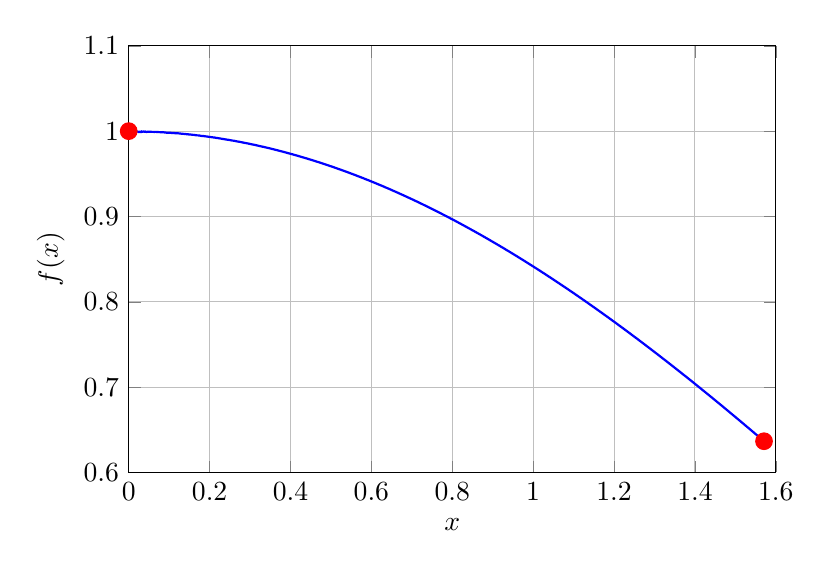
\begin{tikzpicture}
    \begin{axis}[
        width=9.8cm,
        height=7cm,
        xlabel={$x$},
        ylabel={$f(x)$},
        xmin=0, xmax=1.6,
        ymin=0.6, ymax=1.1,
        grid=major
    ]
    
    % Plot (d): f(x) = sin(x)/x
    \addplot[blue, thick, samples=1000, domain=0.01:1.57] {sin(deg(x))/x};
    
    % Mark the endpoints
    \addplot[only marks, mark=*, mark size=3pt, red] coordinates {
        (0, 1) (1.5708, 0.6366)
    };
    
    \end{axis}
\end{tikzpicture}
\caption{Problem 5.2(d): The sinc function $f(x) = \frac{\sin x}{x}$ on the interval $[0,\pi/2]$. The red dots mark the endpoints, showing the maximum at $x=0$ and minimum at $x=\pi/2$.}
\end{figure}

\bigskip\noindent\textbf{Solution:}
\(\,(a)\,\) $f'(x)=3x^2+a$. If $a\ge 0$ then $f'>0$ on $\mathbb{R}$ and $f$ is strictly increasing (no extrema). If $a<0$, set $r=\sqrt{-a/3}$. Then $f'>0$ on $(-\infty,-r)\cup(r,\infty)$ and $f'<0$ on $(-r,r)$, so $f$ has a local maximum at $x=-r$ and a local minimum at $x=r$. Using $a=-3r^2$,
\[f(\pm r)=\pm r^3-3r^2(\pm r)+b=b\mp 2r^3.\]
\(\,(b)\,\) On $(-\infty,-3)$ and $(3,\infty)$, $f'(x)=\dfrac{2x}{x^2-9}$ has the sign of $x$. Thus $f$ decreases on $(-\infty,-3)$ and increases on $(3,\infty)$. No maxima/minima on the domain; $f\to-\infty$ as $x\to\pm3$.\newline
\(\,(c)\,\) On $[0,1]$, $f(x)=x^{2/3}(x-1)^4>0$ except at $0,1$. Writing $\ln f=\tfrac23\ln x+4\ln(1-x)$ gives
\[\frac{f'}{f}=\frac{2}{3x}-\frac{4}{1-x}=0\iff x=\frac17.\]
Thus $f$ increases on $(0,1/7)$, decreases on $(1/7,1)$, with a unique interior maximum at $x=1/7$, and zeros (hence minima) at $0$ and $1$.\newline
\(\,(d)\,\) For $x>0$, $f'(x)=\dfrac{x\cos x-\sin x}{x^2}<0$ on $(0,\pi/2]$ (since $\tan x> x$ there). Hence $f$ is decreasing on $[0,\pi/2]$; its maximum is $f(0)=1$ and its minimum is $f(\pi/2)=2/\pi$.\qed


\begin{problembox}[5.3: Polynomial Interpolation]
Find a polynomial \( f \) of lowest possible degree such that
\[ f(x_1) = a_1, \quad f(x_2) = a_2, \quad f'(x_1) = b_1, \quad f'(x_2) = b_2, \]
where \( x_1 \neq x_2 \) and \( a_1, a_2, b_1, b_2 \) are given real numbers.
\end{problembox}

\noindent\textbf{Strategy:} Use Hermite interpolation. With 4 conditions (2 function values and 2 derivative values), the minimal degree is 3. Use the Hermite basis polynomials that satisfy the interpolation conditions by construction.

\bigskip\noindent\textbf{Solution:}
The minimal degree is \textbf{$3$} (Hermite data at two nodes). The unique cubic can be written with Hermite basis polynomials:
\[\begin{aligned}
f(x)&=a_1 H_{10}(x)+a_2 H_{20}(x)+b_1 H_{11}(x)+b_2 H_{21}(x),\\
H_{10}(x)&=\Big(1-2\frac{x-x_1}{x_2-x_1}\Big)\Big(\frac{x-x_2}{x_1-x_2}\Big)^2,\quad H_{11}(x)=(x-x_1)\Big(\frac{x-x_2}{x_1-x_2}\Big)^2,\\
H_{20}(x)&=\Big(1-2\frac{x-x_2}{x_1-x_2}\Big)\Big(\frac{x-x_1}{x_2-x_1}\Big)^2,\quad H_{21}(x)=(x-x_2)\Big(\frac{x-x_1}{x_2-x_1}\Big)^2.
\end{aligned}\]
Then $f(x_i)=a_i$ and $f'(x_i)=b_i$ follow by construction.\qed


\begin{problembox}[5.4: Smoothness of Exponential Function]
Define \( f \) as follows: \( f(x) = e^{-1/x^2} \) if \( x \neq 0, f(0) = 0 \). Show that
a) \( f \) is continuous for all \( x \).
b) \( f^{(n)} \) is continuous for all \( x \), and that \( f^{(n)}(0) = 0, (n = 1, 2, \ldots ) \).
\end{problembox}

\noindent\textbf{Strategy:} Show that \( f \) is smooth everywhere except at 0, then use the fact that \( e^{-1/x^2} \) decays faster than any power of \( x \) as \( x \to 0 \) to prove that all derivatives exist and are continuous at 0.

% Plot for Problem 5.4: Smoothness of exponential function
\begin{figure}[h]
\centering
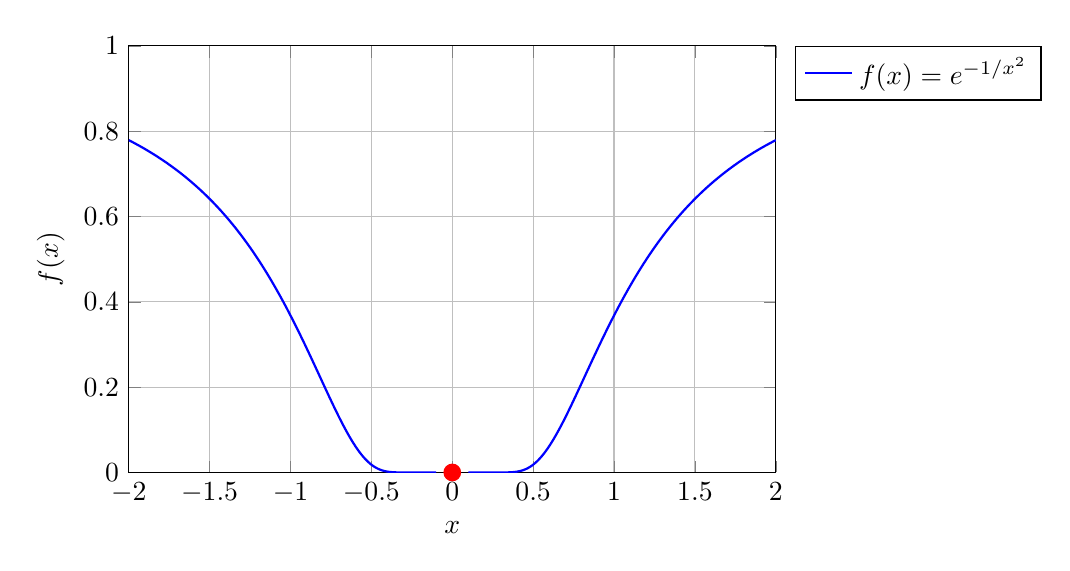
\begin{tikzpicture}
    \begin{axis}[
        width=9.8cm,
        height=7cm,
        xlabel={$x$},
        ylabel={$f(x)$},
        xmin=-2, xmax=2,
        ymin=0, ymax=1,
        grid=major,
        legend pos=outer north east
    ]
    
    % Plot the main function
    \addplot[blue, thick, samples=1000, domain=-2:-0.1] {exp(-1/(x^2))};
    \addplot[blue, thick, samples=1000, domain=0.1:2] {exp(-1/(x^2))};
    \addlegendentry{$f(x) = e^{-1/x^2}$}
    
    % Mark the point at x=0
    \addplot[only marks, mark=*, mark size=3pt, red] coordinates {
        (0, 0)
    };
    
    % Add a small gap to show discontinuity in plotting
    \addplot[white, thick] coordinates {(-0.05, 0) (0.05, 0)};
    
    \end{axis}
\end{tikzpicture}
\caption{Problem 5.4: The function $f(x) = e^{-1/x^2}$ showing its smoothness at $x=0$. The function approaches 0 as $x \to 0$ and is infinitely differentiable everywhere.}
\end{figure}

\noindent\textbf{Proof.}
For $x\ne 0$, $f$ is $C^{\infty}$. At $0$, $f(x)\to 0$ as $x\to 0$, so $f$ is continuous. Moreover, for each $n\ge 1$ there is a polynomial $P_n(1/x)$ such that $f^{(n)}(x)=P_n(1/x)\,e^{-1/x^2}$ for $x\ne 0$. Since $e^{-1/x^2}$ decays faster than any power as $x\to 0$, $\lim_{x\to 0}f^{(n)}(x)=0$. Define $f^{(n)}(0)=0$; then $f^{(n)}$ is continuous for all $n$.



\begin{problembox}[5.5: Derivatives of Trigonometric Functions]
Define \( f, g, \) and \( h \) as follows: \( f(0) = g(0) = h(0) = 0 \) and, if \( x \neq 0, f(x) = \sin (1/x), g(x) = x \sin (1/x), h(x) = x^2 \sin (1/x) \). Show that
a) \( f'(x) = -1/x^2 \cos (1/x), \) if \( x \neq 0; \quad f'(0) \) does not exist.
b) \( g'(x) = \sin (1/x) - 1/x \cos (1/x), \) if \( x \neq 0; \quad g'(0) \) does not exist.
c) \( h'(x) = 2x \sin (1/x) - \cos (1/x), \) if \( x \neq 0; \quad h'(0) = 0; \lim_{x \to 0} h'(x) \) does not exist.
\end{problembox}

\noindent\textbf{Strategy:} Use the chain rule and product rule to compute derivatives for \( x \neq 0 \). For \( x = 0 \), use the definition of the derivative and analyze the behavior of the difference quotient as \( x \to 0 \).

% Plot for Problem 5.5: Trigonometric functions with 1/x argument
\begin{figure}[h]
\centering
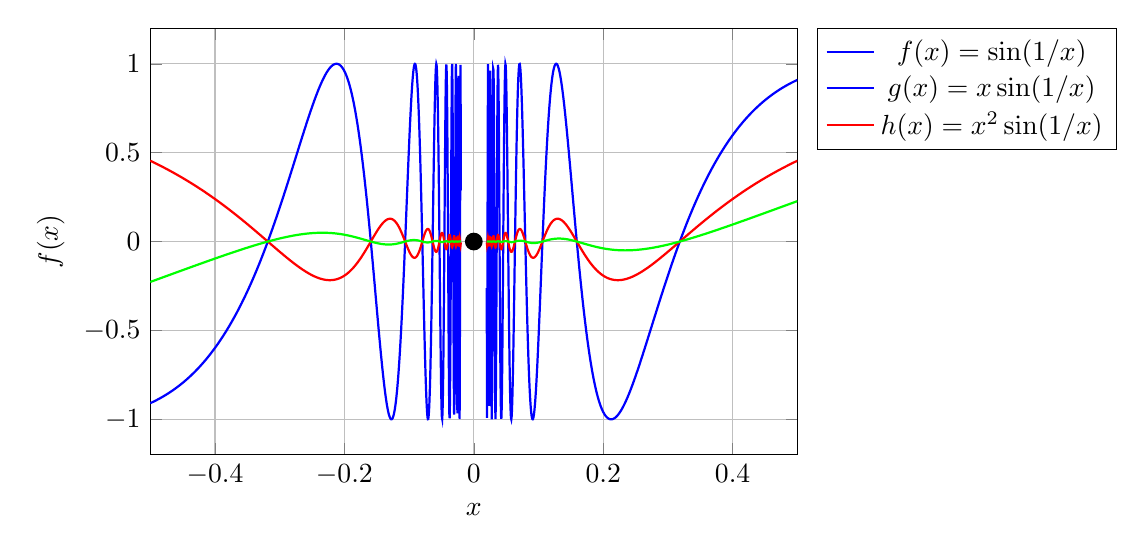
\begin{tikzpicture}
    \begin{axis}[
        width=9.8cm,
        height=7cm,
        xlabel={$x$},
        ylabel={$f(x)$},
        xmin=-0.5, xmax=0.5,
        ymin=-1.2, ymax=1.2,
        grid=major,
        legend pos=outer north east
    ]
    
    % Plot f(x) = sin(1/x)
    \addplot[blue, thick, samples=1000, domain=-0.5:-0.02] {sin(deg(1/x))};
    \addplot[blue, thick, samples=1000, domain=0.02:0.5] {sin(deg(1/x))};
    \addlegendentry{$f(x) = \sin(1/x)$}
    
    % Plot g(x) = x*sin(1/x)
    \addplot[red, thick, samples=1000, domain=-0.5:-0.02] {x*sin(deg(1/x))};
    \addplot[red, thick, samples=1000, domain=0.02:0.5] {x*sin(deg(1/x))};
    \addlegendentry{$g(x) = x\sin(1/x)$}
    
    % Plot h(x) = x^2*sin(1/x)
    \addplot[green, thick, samples=1000, domain=-0.5:-0.02] {x^2*sin(deg(1/x))};
    \addplot[green, thick, samples=1000, domain=0.02:0.5] {x^2*sin(deg(1/x))};
    \addlegendentry{$h(x) = x^2\sin(1/x)$}
    
    % Mark the point at x=0
    \addplot[only marks, mark=*, mark size=3pt, black] coordinates {
        (0, 0)
    };
    
    \end{axis}
\end{tikzpicture}
\caption{Problem 5.5: Trigonometric functions with $1/x$ argument near $x=0$. The functions show different behavior: $f(x) = \sin(1/x)$ oscillates without bound, $g(x) = x\sin(1/x)$ is bounded but not differentiable at 0, and $h(x) = x^2\sin(1/x)$ is differentiable at 0.}
\end{figure}

\noindent\textbf{Proof.}
For $x\ne 0$, use the chain and product rules:
\[f'(x)=\cos(1/x)\cdot(-1/x^2),\quad g'(x)=\sin(1/x)+x\cos(1/x)\cdot(-1/x^2),\]
\[h'(x)=2x\sin(1/x)+x^2\cos(1/x)\cdot(-1/x^2)=2x\sin(1/x)-\cos(1/x).\]
At $0$, $\lim_{x\to 0}\dfrac{\sin(1/x)}{x}$ does not exist, so $f'(0)$ and $g'(0)$ do not exist. For $h$, $\dfrac{h(x)-h(0)}{x}=x\sin(1/x)\to 0$, so $h'(0)=0$. But $h'(x)$ oscillates without limit as $x\to 0$.



\begin{problembox}[5.6: Leibnitz's Formula]
Derive Leibnitz's formula for the nth derivative of the product \( h \) of two functions \( f \) and \( g \):
\[ h^{(n)}(x) = \sum_{k=0}^{n} \binom{n}{k} f^{(k)}(x)g^{(n-k)}(x), \quad \text{where} \quad \binom{n}{k} = \frac{n!}{k!(n-k)!}. \]
\end{problembox}

\noindent\textbf{Strategy:} Use mathematical induction. The base case \( n = 1 \) is the product rule. For the inductive step, differentiate the formula for \( h^{(n)} \) and use the binomial coefficient identity \( \binom{n}{k-1} + \binom{n}{k} = \binom{n+1}{k} \).

\noindent\textbf{Proof.}
Induct on $n$. For $n=1$ the statement is the product rule. Assume true for $n$. Differentiate
\[h^{(n)}=\sum_{k=0}^n\binom{n}{k}f^{(k)}g^{(n-k)}\]
to get
\[h^{(n+1)}=\sum_{k=0}^n\binom{n}{k}f^{(k+1)}g^{(n-k)}+\sum_{k=0}^n\binom{n}{k}f^{(k)}g^{(n-k+1)},\]
reindex and use $\binom{n}{k-1}+\binom{n}{k}=\binom{n+1}{k}$ to obtain the desired formula for $n+1$.



\begin{problembox}[5.7: Relations for Derivatives]
Let \( f \) and \( g \) be two functions defined and having finite third-order derivatives \( f''(x) \) and \( g''(x) \) for all \( x \) in \( \mathbb{R} \). If \( f(x)g(x) = 1 \) for all \( x \), show that the relations in (a), (b), (c), and (d) hold at those points where the denominators are not zero:
a) \( f'(x)/f(x) + g'(x)/g(x) = 0 \).
b) \( f''(x)/f'(x) - 2f'(x)/f(x) - g''(x)/g'(x) = 0 \).
c) \( \frac{f'''(x)}{f'(x)} - 3\frac{f'(x)g''(x)}{f(x)g'(x)} - 3\frac{f''(x)}{f(x)} - \frac{g'''(x)}{g'(x)} = 0 \).
d) \( \frac{f'''(x)}{f'(x)} - \frac{3}{2}\left(\frac{f''(x)}{f'(x)}\right)^2 = \frac{g'''(x)}{g'(x)} - \frac{3}{2}\left(\frac{g''(x)}{g'(x)}\right)^2 \).

NOTE. The expression which appears on the left side of (d) is called the Schwarzian derivative of \( f \) at \( x \).
e) Show that \( f \) and \( g \) have the same Schwarzian derivative if
\[ g(x) = [af(x) + b][cf(x) + d], \text{where} ad - bc \neq 0. \]
\end{problembox}

\noindent\textbf{Strategy:} Start with the relation \( f(x)g(x) = 1 \) and take logarithms to get (a). Differentiate this relation repeatedly to obtain (b) and (c). For (d), use the fact that the Schwarzian derivative is invariant under Möbius transformations.

\noindent\textbf{Proof.}
Since $fg\equiv 1$, $(\ln f)'+(\ln g)'=0$, which gives (a): $f'/f+g'/g=0$. Differentiating (a) and simplifying yields (b). Repeating once more yields (c). For (d), differentiate $\dfrac{f''}{f'}-\dfrac{3}{2}\Big(\dfrac{f''}{f'}\Big)^{\!2}$ and use (a)–(c) to see the derivatives of the two sides agree and the values coincide at one point, hence they are equal. For (e), interpreting $g$ as the fractional linear transform $g=\dfrac{af+b}{cf+d}$ (with $ad-bc\ne 0$), the Schwarzian derivative is invariant under Möbius transformations, so $Sf\equiv Sg$.



\begin{problembox}[5.8: Derivative of a Determinant]
Let \( f_1, f_2, g_1, g_2 \) be four functions having derivatives in \( (a, b) \). Define \( F \) by means of the determinant
\[ F(x) = \begin{vmatrix}
f_1(x) & f_2(x) \\
g_1(x) & g_2(x)
\end{vmatrix}, \quad \text{if} x \in (a, b). \]
a) Show that \( F'(x) \) exists for each \( x \) in \( (a, b) \) and that
\[ F'(x) = \begin{vmatrix}
f_1'(x) & f_2'(x) \\
g_1(x) & g_2(x)
\end{vmatrix} + \begin{vmatrix}
f_1(x) & f_2(x) \\
g_1'(x) & g_2'(x)
\end{vmatrix}. \]
b) State and prove a more general result for nth order determinants.
\end{problembox}

\noindent\textbf{Strategy:} Use the multilinearity of determinants and the product rule. For a 2×2 determinant, expand it and differentiate term by term. For the general case, use the fact that determinants are multilinear in their rows.

\bigskip\noindent\textbf{Solution:}
By the product rule on the bilinear expansion of the $2\times2$ determinant,
\[\frac{d}{dx}\det\begin{pmatrix}f_1&f_2\\ g_1&g_2\end{pmatrix}=\det\begin{pmatrix}f_1'&f_2'\\ g_1&g_2\end{pmatrix}+\det\begin{pmatrix}f_1&f_2\\ g_1'&g_2'\end{pmatrix}.\]
For an $n\times n$ determinant, multilinearity in the rows gives $\big(\det F\big)'=\sum_{j=1}^{n}\det(F\text{ with the $j$th row differentiated}).$\qed


\begin{problembox}[5.9: Wronskian and Linear Dependence]
Given \( n \) functions \( f_1, \ldots, f_n \), each having nth order derivatives in \( (a, b) \). A function \( W \), called the Wronskian of \( f_1, \ldots, f_n \), is defined as follows: For each \( x \) in \( (a, b) \), \( W(x) \) is the value of the determinant of order \( n \) whose element in the \( k \)th row and \( m \)th column is \( f_m^{(k-1)}(x) \), where \( k = 1, 2, \ldots, n \) and \( m = 1, 2, \ldots, n \). [The expression \( f_m^{(0)}(x) \) is written for \( f_m(x) \).]
a) Show that \( W'(x) \) can be obtained by replacing the last row of the determinant defining \( W(x) \) by the \( n \)th derivatives \( f_1^{(n)}(x), \ldots, f_n^{(n)}(x) \).
b) Assuming the existence of \( n \) constants \( c_1, \ldots, c_n \), not all zero, such that \( c_1 f_1(x) + \cdots + c_n f_n(x) = 0 \) for every \( x \) in \( (a, b) \), show that \( W(x) = 0 \) for each \( x \) in \( (a, b) \).

NOTE. A set of functions satisfying such a relation is said to be a linearly dependent set on \( (a, b) \).

c) The vanishing of the Wronskian throughout \( (a, b) \) is necessary, but not sufficient, for linear dependence of \( f_1, \ldots, f_n \). Show that in the case of two functions, if the Wronskian vanishes throughout \( (a, b) \) and if one of the functions does not vanish in \( (a, b) \), then they form a linearly dependent set in \( (a, b) \).
\end{problembox}

\noindent\textbf{Strategy:} For (a), use the result from Problem 5.8 about differentiating determinants. For (b), use the linear dependence relation to show that one row is a linear combination of the others. For (c), use the quotient rule to show that the ratio of the two functions is constant.

\bigskip\noindent\textbf{Solution:}
(a) Differentiate the determinant by the rule in 5.8: only the last row changes to $\big(f_1^{(n)}(x),\dots,f_n^{(n)}(x)\big)$. (b) If $\sum c_m f_m\equiv 0$ with some $c_m$ not all $0$, then each row of the Wronskian is a linear combination of the others with the same coefficients, so the determinant vanishes identically. (c) For two functions, $W=f_1 f_2'-f_1'f_2\equiv 0$ on $(a,b)$ and, say, $f_2\ne 0$ on $(a,b)$. Then $(f_1/f_2)'=\dfrac{f_1'f_2-f_1 f_2'}{f_2^2}=0$, so $f_1/f_2$ is constant and the pair is linearly dependent.\qed

\section{The Mean-Value Theorem}

\subsection*{Definitions and Theorems}

\begin{theorem}[Rolle's Theorem]
If $f$ is continuous on $[a,b]$, differentiable on $(a,b)$, and $f(a) = f(b)$, then there exists $c \in (a,b)$ such that $f'(c) = 0$.
\end{theorem}

\begin{theorem}[Mean Value Theorem]
If $f$ is continuous on $[a,b]$ and differentiable on $(a,b)$, then there exists $c \in (a,b)$ such that
\[ f'(c) = \frac{f(b) - f(a)}{b - a} \]
\end{theorem}

\begin{theorem}[Cauchy's Mean Value Theorem]
If $f$ and $g$ are continuous on $[a,b]$ and differentiable on $(a,b)$, and $g'(x) \neq 0$ for all $x \in (a,b)$, then there exists $c \in (a,b)$ such that
\[ \frac{f'(c)}{g'(c)} = \frac{f(b) - f(a)}{g(b) - g(a)} \]
\end{theorem}

\begin{theorem}[Generalized Mean Value Theorem]
If $f$ has a finite $n$th derivative in $[a,b]$ and $f^{(k)}(a) = 0$ for $k = 0, 1, \ldots, n-1$, then there exists $c \in (a,b)$ such that
\[ f^{(n)}(c) = \frac{n!}{(b-a)^n} f(b) \]
\end{theorem}

\begin{theorem}[Taylor's Theorem with Lagrange Remainder]
If $f$ has a finite $(n+1)$th derivative in $[a,b]$, then for any $x \in [a,b]$,
\[ f(x) = \sum_{k=0}^{n} \frac{f^{(k)}(a)}{k!} (x-a)^k + \frac{f^{(n+1)}(c)}{(n+1)!} (x-a)^{n+1} \]
where $c$ is some point between $a$ and $x$.
\end{theorem}

\begin{theorem}[Taylor's Theorem with Cauchy Remainder]
If $f$ has a finite $(n+1)$th derivative in $[a,b]$, then for any $x \in [a,b]$,
\[ f(x) = \sum_{k=0}^{n} \frac{f^{(k)}(a)}{k!} (x-a)^k + \frac{(x-a)(x-c)^n}{n!} f^{(n+1)}(c) \]
where $c$ is some point between $a$ and $x$.
\end{theorem}

\begin{theorem}[L'Hôpital's Rule]
If $f$ and $g$ are differentiable on $(a,b)$ except possibly at $c \in (a,b)$, $\lim_{x \to c} f(x) = \lim_{x \to c} g(x) = 0$ or $\pm\infty$, and $\lim_{x \to c} \frac{f'(x)}{g'(x)}$ exists, then
\[ \lim_{x \to c} \frac{f(x)}{g(x)} = \lim_{x \to c} \frac{f'(x)}{g'(x)} \]
\end{theorem}

\begin{problembox}[5.10: Infinite Limit and Derivative]
Given a function \( f \) defined and having a finite derivative in \( (a, b) \) and such that \( \lim_{x \to b^-} f(x) = +\infty \). Prove that \( \lim_{x \to b^-} f'(x) \) either fails to exist or is infinite.
\end{problembox}

\noindent\textbf{Strategy:} Use proof by contradiction. Assume the limit of \( f' \) exists and is finite, then use the Mean Value Theorem to derive a contradiction with the fact that \( f(x) \to +\infty \) as \( x \to b^- \).

\bigskip\noindent\textbf{Solution:}
Suppose $\lim_{x\to b^-}f(x)=+\infty$ and $\lim_{x\to b^-}f'(x)=L\in\mathbb{R}$. Fix $h>0$ small, pick $x$ close to $b$; by the mean value theorem there is $\xi\in(x,b)$ with $\dfrac{f(b-h)-f(x)}{b-h-x}=f'(\xi)$. Letting $x\to b^-$ forces the left side to $-\infty$ while the right tends to $L$, a contradiction. Hence the limit of $f'$ cannot be finite; it either diverges or fails to exist.\qed


\begin{problembox}[5.11: Mean-Value Theorem and Theta]
Show that the formula in the Mean-Value Theorem can be written as follows:
\[ \frac{f(x+h)-f(x)}{h} = f'(x+\theta h), \]
where \( 0 < \theta < 1 \). Determine \( \theta \) as a function of \( x \) and \( h \) when 
a) \( f(x) = x^2 \), 
b) \( f(x) = x^3 \), 
c) \( f(x) = e^x \), 
d) \( f(x) = \log x, \quad x > 0 \).

Keep \( x \neq 0 \) fixed, and find \( \lim_{h \to 0} \theta \) in each case.
\end{problembox}

\noindent\textbf{Strategy:} Use the Mean Value Theorem to express the difference quotient in terms of the derivative at an intermediate point. For each specific function, compute the difference quotient and solve for \( \theta \) in terms of \( x \) and \( h \).

\bigskip\noindent\textbf{Solution:}
By the mean value theorem, for each $h\ne 0$ there is $\theta\in(0,1)$ with $\dfrac{f(x+h)-f(x)}{h}=f'(x+\theta h)$. Compute $\theta$ casewise:
\[\begin{aligned}
f(x)=x^2:&\frac{(x+h)^2-x^2}{h}=2x+h=2(x+\theta h)\Rightarrow\theta=\tfrac12.\\
f(x)=x^3:&\frac{(x+h)^3-x^3}{h}=3x^2+3xh+h^2=3(x+\theta h)^2,\\
& \text{so }\theta=\frac{-x+\sqrt{x^2+xh+\tfrac13 h^2}}{h}\in(0,1).\\
f(x)=e^x:&\frac{e^{x+h}-e^x}{h}=e^{x+\theta h}\Rightarrow \theta=\frac1h\log\frac{e^h-1}{h}.\\
f(x)=\log x\,(x>0):&\frac{\log(x+h)-\log x}{h}=\frac{1}{x+\theta h} \\
& \Rightarrow \theta=\frac{1}{h}\Big(\frac{h}{\log(1+h/x)}-x\Big).
\end{aligned}\]
Fix $x\ne 0$. In each case, expanding for small $h$ shows $\lim_{h\to 0}\theta=\tfrac12$.\qed


\begin{problembox}[5.12: Cauchy's Mean-Value Theorem]
Take \( f(x) = 3x^4 - 2x^3 - x^2 + 1 \) and \( g(x) = 4x^3 - 3x^2 - 2x \) in Theorem 5.20. Show that \( f'(x)/g'(x) \) is never equal to the quotient \( [f(1) - f(0)]/[g(1) - g(0)] \) if \( 0 < x \leq 1 \). How do you reconcile this with the equation
\[ \frac{f(b) - f(a)}{g(b) - g(a)} = \frac{f'(x_1)}{g'(x_1)}, \quad a < x_1 < b, \]
obtainable from Theorem 5.20 when \( n = 1 \)?
\end{problembox}

\noindent\textbf{Strategy:} Compute the specific values and show that the ratio form of Cauchy's theorem fails when \( g'(x_1) = 0 \). The correct interpretation is that the cross-product form \( (f(b) - f(a))g'(x_1) = (g(b) - g(a))f'(x_1) \) holds.

\bigskip\noindent\textbf{Solution:}
Compute $f(1)-f(0)=0$ and $g(1)-g(0)\ne 0$, hence the quotient is $0$. On $(0,1]$, $f'(x)=2x(6x^2-3x-1)$ and $g'(x)=2(6x^2-3x-1)$ vanish at the same point $x_0=\dfrac{3+\sqrt{33}}{12}\in(0,1]$, so $f'(x)/g'(x)$ is never $0$ for $x\in(0,1]$. This does not contradict Cauchy's theorem: the correct conclusion is $(f(1)-f(0))g'(x_1)=(g(1)-g(0))f'(x_1)$ for some $x_1\in(0,1)$, which holds at $x_1=x_0$ (both sides are $0$). The "ratio" form fails there because $g'(x_1)=0$.\qed


\begin{problembox}[5.13: Special Cases of Mean-Value Theorem]
In each of the following special cases of Theorem 5.20, take \( n = 1 \), \( c = a \), \( x = b \), and show that \( x_1 = (a + b)/2 \).

a) \( f(x) = \sin x, \quad g(x) = \cos x; \) 
b) \( f(x) = e^x, \quad g(x) = e^{-x} \).

Can you find a general class of such pairs of functions \( f \) and \( g \) for which \( x_1 \) will always be \( (a + b)/2 \) and such that both examples (a) and (b) are in this class?
\end{problembox}

\noindent\textbf{Strategy:} Apply Cauchy's Mean Value Theorem to each pair and use trigonometric identities or exponential properties to show that the intermediate point must be the midpoint. Look for functions that satisfy certain differential equations.

\bigskip\noindent\textbf{Solution:}
For (a), with $f=\sin,\ g=\cos$, Cauchy's theorem gives $(\sin b-\sin a)\,(-\sin x_1)=(\cos b-\cos a)\,\cos x_1$. Using sum-to-product identities this reduces to $\sin\big(\tfrac{a+b}{2}-x_1\big)=0$, hence $x_1=\tfrac{a+b}{2}$. For (b), $f=e^x,\ g=e^{-x}$ yields $e^b-e^a=(e^{-a}-e^{-b})e^{2x_1}$, whence $x_1=\tfrac{a+b}{2}$. A general class: pairs $f,g$ solving a linear ODE $y''+\lambda y=0$ (e.g., $\sin,\cos$) or $y''-\lambda y=0$ (e.g., $e^x,e^{-x}$) have this midpoint property.\qed


\begin{problembox}[5.14: Limit of a Sequence]
Given a function \( f \) defined and having a finite derivative \( f' \) in the half-open interval \( 0 < x \leq 1 \) and such that \( |f'(x)| < 1 \). Define \( a_n = f(1/n) \) for \( n = 1, 2, 3, \ldots \), and show that \( \lim_{n \to \infty} a_n \) exists. Hint. Cauchy condition.
\end{problembox}

\noindent\textbf{Strategy:} Use the Mean Value Theorem to bound the difference between terms in the sequence, then apply the Cauchy criterion for convergence.

\bigskip\noindent\textbf{Solution:}
For $m,n$, by the mean value theorem there is $\xi$ between $1/m$ and $1/n$ with
\[|a_m-a_n|=|f(1/m)-f(1/n)|\le |f'(\xi)|\,\Big|\frac1m-\frac1n\Big|\le \alpha\,\Big|\frac1m-\frac1n\Big|,\]
for some $\alpha<1$. Hence $(a_n)$ is Cauchy, so $\lim a_n$ exists.\qed


\begin{problembox}[5.15: Limit of Derivative]
Assume that \( f \) has a finite derivative at each point of the open interval \( (a, b) \). Assume also that \( \lim_{x \to c} f'(x) \) exists and is finite for some interior point \( c \). Prove that the value of this limit must be \( f'(c) \).
\end{problembox}

\noindent\textbf{Strategy:} Use Cauchy's Mean Value Theorem to relate the difference quotient to the derivative at an intermediate point, then take the limit as \( x \to c \).

\bigskip\noindent\textbf{Solution:}
We have
\[\frac{f(x)-f(c)}{x-c}-f'(x)=\frac{f(x)-f(c)-(x-c)f'(x)}{x-c}.\]
By Cauchy's mean value theorem applied to $F(t)=f(t)-f(c)-(t-c)f'(x)$ and $G(t)=t-c$, there is $\xi$ between $x$ and $c$ such that the quotient equals $\dfrac{f'(\xi)-f'(x)}{1}$. Letting $x\to c$ gives $\dfrac{f(x)-f(c)}{x-c}\to L$, hence $f'(c)=L$.\qed


\begin{problembox}[5.16: Extension of Derivative]
Let \( f \) be continuous on \( (a, b) \) with a finite derivative \( f' \) everywhere in \( (a, b) \), except possibly at \( c \). If \( \lim_{x \to c} f'(x) \) exists and has the value \( A \), show that \( f'(c) \) must also exist and have the value \( A \).
\end{problembox}

\noindent\textbf{Strategy:} Use the Mean Value Theorem to relate the difference quotient to the derivative at an intermediate point, then use the continuity of \( f \) and the limit of \( f' \) to show that the difference quotient tends to \( A \).

\bigskip\noindent\textbf{Solution:}
As in 5.15, for $x\ne c$ choose $\xi$ between $x$ and $c$ to get
\[\frac{f(x)-f(c)}{x-c}-A=f'(\xi)-A.\]
Let $x\to c$; then $\xi\to c$ and $f'(\xi)\to A$ by hypothesis, so the difference quotient tends to $A$. Thus $f'(c)$ exists and equals $A$.\qed


\begin{problembox}[5.17: Monotonicity of Quotient]
Let \( f \) be continuous on \( [0, 1] \), \( f(0) = 0 \), \( f'(x) \) finite for each \( x \) in \( (0, 1) \). Prove that if \( f' \) is an increasing function on \( (0, 1) \), then so too is the function \( g \) defined by the equation \( g(x) = f(x)/x \).
\end{problembox}

\noindent\textbf{Strategy:} Use Cauchy's Mean Value Theorem to compare \( g(v) - g(u) \) for \( 0 < u < v \leq 1 \), and use the fact that \( f' \) is increasing to show that this difference is nonnegative.

\bigskip\noindent\textbf{Solution:}
For $0<u<v\le 1$, apply Cauchy's mean value theorem to $f$ and $x\mapsto x$ on $[u,v]$ to get
\[\frac{f(v)-f(u)}{v-u}=f'(\xi)\quad(\xi\in(u,v)).\]
Then
\begin{align*}
\frac{f(v)}{v}-\frac{f(u)}{u}=&\frac{uf(v)-vf(u)}{uv}=\frac{u[v f'(\xi)-(f(v)-f(u))]}{uv} \\
=& \frac{u(v-\xi)}{uv}\,[f'(\xi)-f'(\eta)]\ge 0,
\end{align*}
using the mean value theorem on $f$ again and the monotonicity of $f'$. Hence $g(x)=f(x)/x$ is increasing.\qed


\begin{problembox}[5.18: Rolle's Theorem Application]
Assume \( f \) has a finite derivative in \( (a, b) \) and is continuous on \( [a, b] \) with \( f(a) = f(b) = 0 \). Prove that for every real \( \lambda \) there is some \( c \) in \( (a, b) \) such that \( f'(c) = \lambda f(c) \). Hint. Apply Rolle's theorem to \( g(x)f(x) \) for a suitable \( g \) depending on \( \lambda \).
\end{problembox}

\noindent\textbf{Strategy:} Choose \( g(x) = e^{-\lambda x} \) so that \( g(x)f(x) \) has the same zeros as \( f \), then apply Rolle's theorem to find a point where the derivative of this product vanishes.

\bigskip\noindent\textbf{Solution:}
Fix $\lambda\in\mathbb{R}$ and set $g(x)=e^{-\lambda x}$. Then $(gf)(a)=(gf)(b)=0$. By Rolle's theorem there is $c\in(a,b)$ with $(gf)'(c)=0$, i.e., $-\lambda e^{-\lambda c}f(c)+e^{-\lambda c}f'(c)=0$, so $f'(c)=\lambda f(c)$.\qed


\begin{problembox}[5.19: Second Derivative and Secant Line]
Assume \( f \) is continuous on \( [a, b] \) and has a finite second derivative \( f'' \) in the open interval \( (a, b) \). Assume that the line segment joining the points \( A = (a, f(a)) \) and \( B = (b, f(b)) \) intersects the graph of \( f \) in a third point \( P \) different from \( A \) and \( B \). Prove that \( f''(c) = 0 \) for some \( c \) in \( (a, b) \).
\end{problembox}

\noindent\textbf{Strategy:} Define \( \phi(x) = f(x) - \ell(x) \) where \( \ell \) is the secant line. Then \( \phi \) has three zeros, so by Rolle's theorem applied twice, there must be a point where \( \phi''(c) = 0 \), which implies \( f''(c) = 0 \).

% Plot for Problem 5.19: Secant line intersecting graph
\begin{figure}[h]
\centering
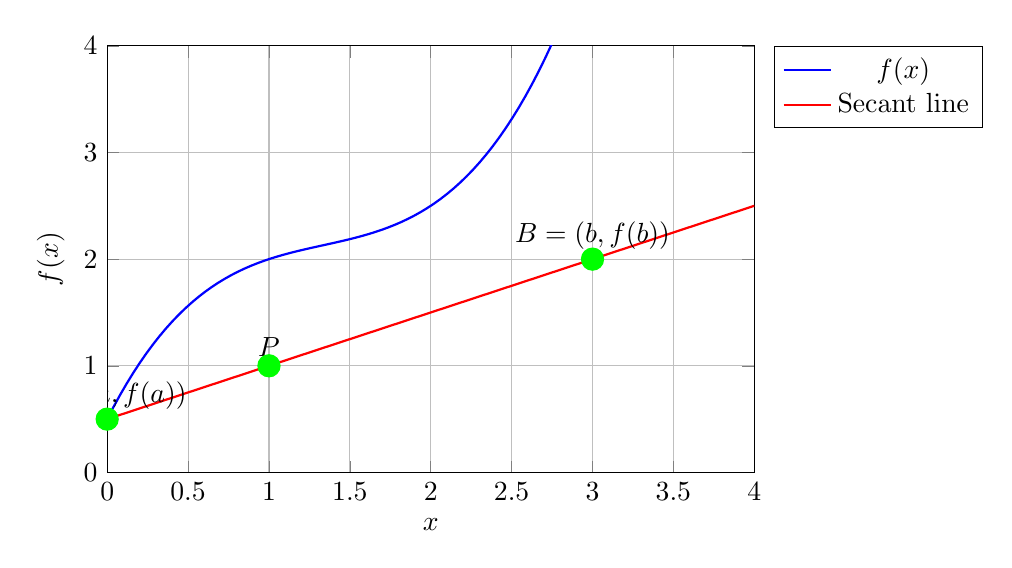
\begin{tikzpicture}
    \begin{axis}[
        width=9.8cm,
        height=7cm,
        xlabel={$x$},
        ylabel={$f(x)$},
        xmin=0, xmax=4,
        ymin=0, ymax=4,
        grid=major,
        legend pos=outer north east
    ]
    
    % Plot a cubic function that intersects the secant line in three points
    \addplot[blue, thick, samples=100, domain=0:4] {0.5*x^3 - 2*x^2 + 3*x + 0.5};
    \addlegendentry{$f(x)$}
    
    % Plot the secant line
    \addplot[red, thick, samples=100, domain=0:4] {0.5*x + 0.5};
    \addlegendentry{Secant line}
    
    % Mark the intersection points
    \addplot[only marks, mark=*, mark size=4pt, green] coordinates {
        (0, 0.5) (1, 1) (3, 2)
    };
    
    % Add labels
    \node[above] at (axis cs: 0, 0.5) {$A = (a, f(a))$};
    \node[above] at (axis cs: 1, 1) {$P$};
    \node[above] at (axis cs: 3, 2) {$B = (b, f(b))$};
    
    \end{axis}
\end{tikzpicture}
\caption{Problem 5.19: A cubic function and its secant line intersecting in three points. The secant line through points $A$ and $B$ intersects the graph of $f$ at a third point $P$, illustrating the geometric condition that leads to $f''(c) = 0$ for some $c \in (a,b)$.}
\end{figure}

\bigskip\noindent\textbf{Solution:}
Let $\ell$ be the secant line through $(a,f(a))$ and $(b,f(b))$, and $\phi=f-\ell$. Then $\phi(a)=\phi(b)=\phi(p)=0$. By Rolle's theorem, there exist $u\in(a,p)$ and $v\in(p,b)$ with $\phi'(u)=\phi'(v)=0$. Applying Rolle again to $\phi'$ on $[u,v]$ yields $c\in(u,v)$ with $\phi''(c)=0$, hence $f''(c)=0$.\qed


\begin{problembox}[5.20: Third Derivative Condition]
If \( f \) has a finite third derivative \( f'' \) in \( [a, b] \) and if
\[ f(a) = f'(a) = f(b) = f'(b) = 0, \]
prove that \( f''(c) = 0 \) for some \( c \) in \( (a, b) \).
\end{problembox}

\noindent\textbf{Strategy:} Use Rolle's theorem twice: first to find a point where \( f' \) vanishes (since \( f(a) = f(b) = 0 \)), then apply Rolle's theorem to \( f' \) on an appropriate subinterval.

\bigskip\noindent\textbf{Solution:}
From $f(a)=f(b)=0$, there exists $s\in(a,b)$ with $f'(s)=0$. Since also $f'(a)=f'(b)=0$, applying Rolle to $f'$ on $[a,s]$ (or $[s,b]$) gives $c$ with $f''(c)=0$.\qed


\begin{problembox}[5.21: Nonnegative Function with Zeros]
Assume \( f \) is nonnegative and has a finite third derivative \( f'' \) in the open interval (0, 1). If \( f(x) = 0 \) for at least two values of \( x \) in (0, 1), prove that \( f''(c) = 0 \) for some \( c \) in (0, 1).
\end{problembox}

\noindent\textbf{Strategy:} Since \( f \) is nonnegative and has zeros at interior points, the derivative must also vanish at these points. Then apply the result from Problem 5.20 to the subinterval between the zeros.

\bigskip\noindent\textbf{Solution:}
Let $u<v$ be two zeros of $f$ in $(0,1)$. Because $f\ge 0$ and $f(u)=0$ at an interior point, necessarily $f'(u)=0$; similarly $f'(v)=0$. Apply 5.20 on $[u,v]$ to conclude that $f''(c)=0$ for some $c\in(u,v)\subset(0,1)$.\qed


\begin{problembox}[5.22: Behavior at Infinity]
Assume \( f \) has a finite derivative in some interval \( (a, +\infty) \).
a) If \( f(x) \to 1 \) and \( f'(x) \to c \) as \( x \to +\infty \), prove that \( c = 0 \).
b) If \( f'(x) \to 1 \) as \( x \to +\infty \), prove that \( f(x)/x \to 1 \) as \( x \to +\infty \).
c) If \( f'(x) \to 0 \) as \( x \to +\infty \), prove that \( f(x)/x \to 0 \) as \( x \to +\infty \).
\end{problembox}

\noindent\textbf{Strategy:} For (a), use the Mean Value Theorem to relate the difference quotient to the derivative. For (b) and (c), consider the function \( g(x) = f(x) - x \) or use integration to bound the growth of \( f \).

\bigskip\noindent\textbf{Solution:}
(a) If $f(x)\to 1$ and $f'(x)\to c$, then for fixed $h>0$ and large $x$, $\dfrac{f(x+h)-f(x)}{h}\to c$ by the mean value theorem, while the numerator $\to 0$. Hence $c=0$. (b) Let $g(x)=f(x)-x$. Then $g'(x)=f'(x)-1\to 0$. For any $\varepsilon>0$, for large $x$, $|g'(t)|<\varepsilon$ for $t\ge x$, so $|g(t)-g(x)|\le \varepsilon|t-x|$. Taking $t=x$ and $t=2x$ shows $|f(2x)-2f(x)|\le \varepsilon x$, which implies $\lim_{x\to\infty}f(x)/x=1$. (c) Similarly, if $f'(x)\to 0$, then for large $x$, $|f(x)-f(0)|\le \int_0^x|f'(t)|dt\le \varepsilon x+C$, so $|f(x)/x|\le \varepsilon+C/x\to 0$.\qed


\begin{problembox}[5.23: Nonexistence of Function]
Let \( h \) be a fixed positive number. Show that there is no function \( f \) satisfying the following three conditions: \( f'(x) \) exists for \( x \geq 0 \), \( f'(0) = 0 \), \( f'(x) \geq h \) for \( x > 0 \).
\end{problembox}

\noindent\textbf{Strategy:} Use proof by contradiction. Assume such a function exists, then use the Mean Value Theorem to show that the difference quotient at 0 must be at least \( h \), contradicting \( f'(0) = 0 \).

\bigskip\noindent\textbf{Solution:}
If $f'(0)=0$ and $f'(x)\ge h>0$ for $x>0$, then for $x>0$, by the mean value theorem there is $\xi\in(0,x)$ with $\dfrac{f(x)-f(0)}{x-0}=f'(\xi)\ge h$. Thus $\liminf_{x\downarrow 0}\dfrac{f(x)-f(0)}{x}\ge h$, contradicting $f'(0)=0$.\qed


\begin{problembox}[5.24: Symmetric Difference Quotients]
If \( h > 0 \) and if \( f'(x) \) exists (and is finite) for every \( x \) in \( (a - h, a + h) \), and if \( f \) is continuous on \( [a - h, a + h] \), show that we have:
a) \( \frac{f(a + h) - f(a - h)}{h} = f'(a + \theta h) + f'(a - \theta h), \quad 0 < \theta < 1; \)
b) \( \frac{f(a + h) - 2f(a) + f(a - h)}{h} = f'(a + \lambda h) - f'(a - \lambda h), \quad 0 < \lambda < 1. \)
c) If \( f''(a) \) exists, show that
\[ f''(a) = \lim_{h \to 0} \frac{f(a + h) - 2f(a) + f(a - h)}{h^2}. \]
d) Give an example where the limit of the quotient in (c) exists but where \( f''(a) \) does not exist.
\end{problembox}

\noindent\textbf{Strategy:} For (a), define \( \phi(t) = f(t) - f(2a - t) \) and apply the Mean Value Theorem. For (b), apply (a) to \( f' \). For (c), use the result from (b) and take the limit. For (d), use a function with a corner at \( a \).

% Plot for Problem 5.24: Symmetric difference quotients
\begin{figure}[h]
\centering
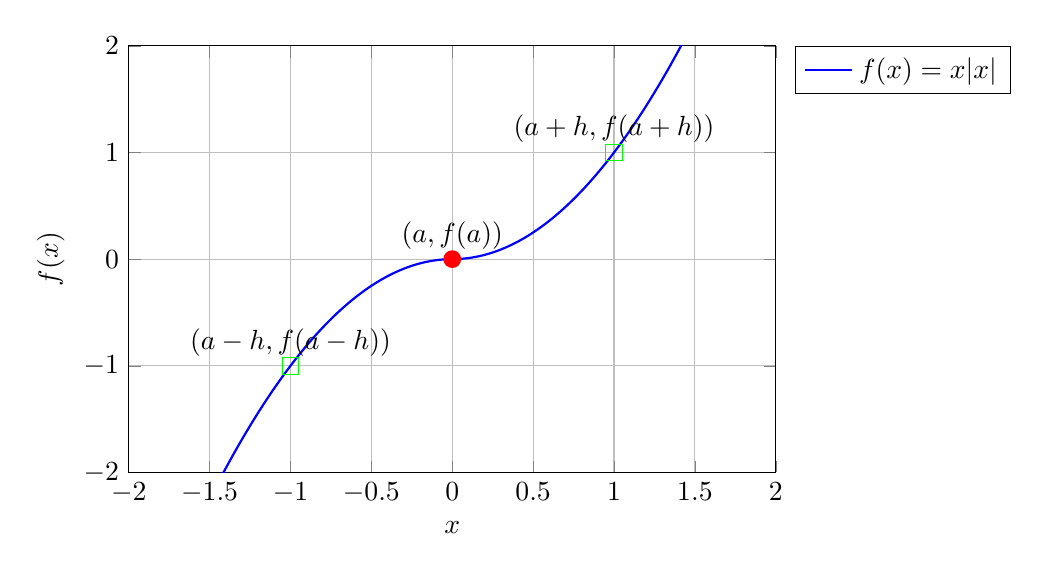
\begin{tikzpicture}
    \begin{axis}[
        width=9.8cm,
        height=7cm,
        xlabel={$x$},
        ylabel={$f(x)$},
        xmin=-2, xmax=2,
        ymin=-2, ymax=2,
        grid=major,
        legend pos=outer north east
    ]
    
    % Plot the example function f(x) = x|x|
    \addplot[blue, thick, samples=100, domain=-2:0] {x*abs(x)};
    \addplot[blue, thick, samples=100, domain=0:2] {x*abs(x)};
    \addlegendentry{$f(x) = x|x|$}
    
    % Mark the point at x=0
    \addplot[only marks, mark=*, mark size=3pt, red] coordinates {
        (0, 0)
    };
    
    % Show symmetric points for h=1
    \addplot[only marks, mark=square, mark size=3pt, green] coordinates {
        (-1, -1) (1, 1)
    };
    
    % Add labels
    \node[above] at (axis cs: -1, -1) {$(a-h, f(a-h))$};
    \node[above] at (axis cs: 1, 1) {$(a+h, f(a+h))$};
    \node[above] at (axis cs: 0, 0) {$(a, f(a))$};
    
    \end{axis}
\end{tikzpicture}
\caption{Problem 5.24: The function $f(x) = x|x|$ showing symmetric difference quotients. This function has a corner at $x=0$ where the second derivative does not exist, but the symmetric second difference quotient has a limit of 0.}
\end{figure}

\bigskip\noindent\textbf{Solution:}
(a) Define $\phi(t)=f(t)-f(2a-t)$. Then $\phi$ is differentiable and by the mean value theorem there is $\theta\in(0,1)$ with
\[\frac{f(a+h)-f(a-h)}{h}=\phi'(a+\theta h)=f'(a+\theta h)+f'(a-\theta h).\]
(b) Apply (a) to $f'$ to get
\[\frac{f'(a+h)-f'(a-h)}{1}=\frac{f(a+h)-2f(a)+f(a-h)}{h}=f'(a+\lambda h)-f'(a-\lambda h).\]
(c) If $f''(a)$ exists, by (b) the symmetric second difference quotient tends to $f''(a)$. (d) Let $f(x)=x|x|$. Then $f''(0)$ does not exist, but
\[\frac{f(h)-2f(0)+f(-h)}{h^2}=\frac{h|h|+(-h)|-h|}{h^2}=0\to 0.\]\qed


\begin{problembox}[5.25: Uniform Differentiability]
Let \( f \) have a finite derivative in \( (a, b) \) and assume that \( c \in (a, b) \). Consider the following condition: For every \( \varepsilon > 0 \) there exists a 1-ball \( B(c; \delta) \), whose radius \( \delta \) depends only on \( \varepsilon \) and not on \( c \), such that if \( x \in B(c; \delta) \), and \( x \neq c \), then
\[ \left| \frac{f(x) - f(c)}{x - c} - f'(c) \right| < \varepsilon. \]
Show that \( f' \) is continuous on \( (a, b) \) if this condition holds throughout \( (a, b) \).
\end{problembox}

\noindent\textbf{Strategy:} Use the uniform condition to show that \( f' \) satisfies the Cauchy criterion for continuity. Fix \( c \) and \( \varepsilon \), then use the condition to bound \( |f'(x) - f'(y)| \) for nearby points \( x \) and \( y \).

\bigskip\noindent\textbf{Solution:}
Fix $c$ and $\varepsilon>0$. By hypothesis choose $\delta$ (depending only on $\varepsilon$) so that for all $x,y\in(a,b)$ with $0<|x-c|,|y-c|<\delta$,
\[\left|\frac{f(x)-f(c)}{x-c}-f'(c)\right|<\tfrac\varepsilon2,\quad \left|\frac{f(y)-f(c)}{y-c}-f'(c)\right|<\tfrac\varepsilon2.\]
Then
\[|f'(x)-f'(y)|\le \left|\frac{f(x)-f(c)}{x-c}-f'(c)\right|+\left|\frac{f(y)-f(c)}{y-c}-f'(c)\right|<\varepsilon.\]
Thus $f'$ is Cauchy (hence continuous) at $c$. Since $c$ was arbitrary, $f'$ is continuous on $(a,b)$.\qed


\begin{problembox}[5.26: Fixed Point Theorem]
Assume \( f \) has a finite derivative in \( (a, b) \) and is continuous on \( [a, b] \), with \( a \leq f(x) \leq b \) for all \( x \) in \( [a, b] \) and \( |f'(x)| \leq \alpha < 1 \) for all \( x \) in \( (a, b) \). Prove that \( f \) has a unique fixed point in \( [a, b] \).
\end{problembox}

\noindent\textbf{Strategy:} Use the Mean Value Theorem to show that \( f \) is a contraction mapping, then apply the contraction mapping theorem or use iteration to find the fixed point.

\bigskip\noindent\textbf{Solution:}
For $x,y\in[a,b]$, by the mean value theorem there exists $\xi$ between $x$ and $y$ with $|f(x)-f(y)|=|f'(\xi)||x-y|\le \alpha|x-y|$. Thus $f$ is a contraction of the complete metric space $[a,b]$, so it has a unique fixed point by the contraction mapping theorem. Alternatively, iterate $x_{n+1}=f(x_n)$ to get a Cauchy sequence converging to the unique fixed point.\qed


\begin{problembox}[5.27: L'Hôpital's Rule Counterexample]
Give an example of a pair of functions \( f \) and \( g \) having finite derivatives in (0, 1), such that
\[ \lim_{x \to 0} \frac{f(x)}{g(x)} = 0, \]
but such that \( \lim_{x \to 0} f'(x)/g'(x) \) does not exist, choosing \( g \) so that \( g'(x) \) is never zero.
\end{problembox}

\noindent\textbf{Strategy:} Use a function like \( f(x) = x^2 \sin(1/x) \) and \( g(x) = x \). The quotient \( f(x)/g(x) \) tends to 0, but \( f'(x)/g'(x) \) oscillates and has no limit.

\bigskip\noindent\textbf{Solution:}
Let $g(x)=x$ and $f(x)=x^2\sin(1/x)$ for $x\in(0,1)$, with $f(0)=g(0)=0$. Then $f(x)/g(x)=x\sin(1/x)\to 0$, while $f'(x)/g'(x)=\big(2x\sin(1/x)-\cos(1/x)\big)/1$ has no limit as $x\to 0$ and $g'(x)=1\ne 0$.\qed


\begin{problembox}[5.28: Generalized L'Hôpital's Rule]
Prove the following theorem: Let \( f \) and \( g \) be two functions having finite nth derivatives in (a, b). For some interior point \( c \) in (a, b), assume that \( f(c) = f'(c) = \cdots = f^{(n-1)}(c) = 0 \), and that \( g(c) = g'(c) = \cdots = g^{(n-1)}(c) = 0 \), but that \( g^{(n)}(x) \) is never zero in (a, b). Show that
\[ \lim_{x \to c} \frac{f(x)}{g(x)} = \frac{f^{(n)}(c)}{g^{(n)}(c)}. \]
NOTE. \( f^{(n)} \) and \( g^{(n)} \) are not assumed to be continuous at \( c \).
\end{problembox}

\noindent\textbf{Strategy:} Use Taylor's theorem with remainder to express \( f(x) \) and \( g(x) \) in terms of their nth derivatives at intermediate points, then take the limit as \( x \to c \).

\bigskip\noindent\textbf{Solution:}
Apply Cauchy's mean value theorem repeatedly or use Taylor's theorem with remainder about $c$. Since $f^{(k)}(c)=g^{(k)}(c)=0$ for $k<n$, we have
\[f(x)=\frac{f^{(n)}(\xi_x)}{n!}(x-c)^n,\quad g(x)=\frac{g^{(n)}(\eta_x)}{n!}(x-c)^n\]
for some $\xi_x,\eta_x\to c$. Hence
\[\lim_{x\to c}\frac{f(x)}{g(x)}=\lim_{x\to c}\frac{f^{(n)}(\xi_x)}{g^{(n)}(\eta_x)}=\frac{f^{(n)}(c)}{g^{(n)}(c)},\]
using the assumed nonvanishing of $g^{(n)}$ near $c$.\qed


\begin{problembox}[5.29: Taylor's Theorem with Remainder]
Show that the formula in Taylor's theorem can also be written as follows:
\[ f(x) = \sum_{k=0}^{n-1} \frac{f^{(k)}(c)}{k!} (x - c)^k + \frac{(x - c)(x - x_1)^{n-1}}{(n - 1)!} f^{(n)}(x_1), \]
where \( x_1 \) is interior to the interval joining \( x \) and \( c \). Let \( 1 - \theta = (x - x_1)/(x - c) \). Show that \( 0 < \theta < 1 \) and deduce the following form of the remainder term (due to Cauchy):
\[ \frac{(1 - \theta)^{n-1}(x - c)^n}{(n - 1)!} f^{(n)}[\theta x + (1 - \theta)c]. \]
\end{problembox}

\noindent\textbf{Strategy:} Start with Cauchy's form of the remainder in Taylor's theorem, then use the relation \( x - x_1 = \theta(x - c) \) to rewrite the remainder in terms of \( \theta \).

\bigskip\noindent\textbf{Solution:}
By Cauchy's form of the remainder, for some $x_1$ between $x$ and $c$,
\[f(x)-\sum_{k=0}^{n-1}\frac{f^{(k)}(c)}{k!}(x-c)^k=\frac{f^{(n)}(x_1)}{(n-1)!}(x-c)^{n-1}(x-x_1).\]
Writing $x-x_1=\theta(x-c)$ with $\theta\in(0,1)$ gives the displayed form and yields Cauchy's remainder
\[\frac{(1-\theta)^{n-1}(x-c)^n}{(n-1)!}\,f^{(n)}\big(\theta x+(1-\theta)c\big).\]\qed

\section{Vector-valued functions}

\subsection*{Definitions and Theorems}

\begin{definition}[Vector-Valued Function]
A vector-valued function is a function $f: \mathbb{R} \to \mathbb{R}^n$ that maps real numbers to vectors in $n$-dimensional space.
\end{definition}

\begin{definition}[Vector-Valued Derivative]
A vector-valued function $f$ is differentiable at $c$ if there exists a vector $f'(c)$ such that
\[ \lim_{h \to 0} \frac{\|f(c + h) - f(c) - f'(c)h\|}{|h|} = 0 \]
\end{definition}

\begin{theorem}[Component-wise Differentiation]
A vector-valued function $f = (f_1, f_2, \ldots, f_n)$ is differentiable at $c$ if and only if each component function $f_i$ is differentiable at $c$, and
\[ f'(c) = (f_1'(c), f_2'(c), \ldots, f_n'(c)) \]
\end{theorem}

\begin{theorem}[Dot Product Rule]
If $f$ and $g$ are differentiable vector-valued functions, then
\[ \frac{d}{dt}(f(t) \cdot g(t)) = f'(t) \cdot g(t) + f(t) \cdot g'(t) \]
\end{theorem}

\begin{theorem}[Constant Norm Implies Orthogonality]
If a vector-valued function $f$ has constant norm $\|f(t)\| = C$ for all $t$, then $f(t) \cdot f'(t) = 0$ for all $t$.
\end{theorem}

\begin{problembox}[5.30: Vector-Valued Differentiability]
If a vector-valued function \( f \) is differentiable at \( c \), prove that
\[ f'(c) = \lim_{h \to 0} \frac{1}{h} [f(c + h) - f(c)]. \]
Conversely, if this limit exists, prove that \( f \) is differentiable at \( c \).
\end{problembox}

\noindent\textbf{Strategy:} For the forward direction, use the definition of differentiability. For the converse, define \( f'(c) \) as the limit and show that it satisfies the definition of differentiability using the \( \varepsilon \)-\( \delta \) argument.

\bigskip\noindent\textbf{Solution:}
If $f$ is differentiable at $c$, the definition gives the limit. Conversely, if the limit exists, define $f'(c)$ to be that limit; the standard $\varepsilon$–$\delta$ argument shows $\|f(c+h)-f(c)-f'(c)h\|=o(|h|)$, i.e., differentiability at $c$.\qed


\begin{problembox}[5.31: Constant Norm and Orthogonality]
A vector-valued function \( f \) is differentiable at each point of (a, b) and has constant norm \( \|f\| \). Prove that \( f(t) \cdot f'(t) = 0 \) on (a, b).
\end{problembox}

\noindent\textbf{Strategy:} Differentiate the equation \( \|f(t)\|^2 = f(t) \cdot f(t) \) using the product rule for the dot product, then use the fact that the derivative of a constant is zero.

\bigskip\noindent\textbf{Solution:}
Differentiate $\|f(t)\|^2=f(t)\cdot f(t)$ to get $\dfrac{d}{dt}\|f(t)\|^2=2 f(t)\cdot f'(t)$. Since the left side is $0$, we obtain $f(t)\cdot f'(t)=0$ on $(a,b)$.\qed


\begin{problembox}[5.32: Solution to Differential Equation]
A vector-valued function \( f \) is never zero and has a derivative \( f' \) which exists and is continuous on \( \mathbb{R} \). If there is a real function \( \lambda \) such that \( f'(t) = \lambda(t)f(t) \) for all \( t \), prove that there is a positive real function \( u \) and a constant vector \( c \) such that \( f(t) = u(t)c \) for all \( t \).
\end{problembox}

\noindent\textbf{Strategy:} Solve the scalar differential equation \( u'(t) = \lambda(t)u(t) \) to find \( u(t) \), then define \( c = f(t)/u(t) \) and show that \( c \) is constant by differentiating this quotient.

\bigskip\noindent\textbf{Solution:}
Let $u$ solve $u'(t)=\lambda(t)u(t)$ with $u(t_0)=1$; then $u(t)=\exp\big(\int_{t_0}^t\!\lambda\big)>0$. Define $c=f/u$. Then $c'(t)=\dfrac{f'(t)u(t)-f(t)u'(t)}{u(t)^2}=0$, so $c$ is constant and $f(t)=u(t)\,c$.\qed


\section{Partial Derivatives}

\subsection*{Definitions and Theorems}

\begin{definition}[Partial Derivative]
The partial derivative of a function $f(x_1, x_2, \ldots, x_n)$ with respect to $x_i$ at a point $(a_1, a_2, \ldots, a_n)$ is defined as
\[ \frac{\partial f}{\partial x_i}(a_1, \ldots, a_n) = \lim_{h \to 0} \frac{f(a_1, \ldots, a_i + h, \ldots, a_n) - f(a_1, \ldots, a_n)}{h} \]
if this limit exists.
\end{definition}

\begin{definition}[Directional Derivative]
The directional derivative of $f$ at a point $a$ in the direction of a unit vector $u$ is defined as
\[ D_u f(a) = \lim_{h \to 0} \frac{f(a + hu) - f(a)}{h} \]
if this limit exists.
\end{definition}

\begin{definition}[Gradient]
The gradient of a function $f$ at a point $a$ is the vector of partial derivatives:
\[ \nabla f(a) = \left(\frac{\partial f}{\partial x_1}(a), \frac{\partial f}{\partial x_2}(a), \ldots, \frac{\partial f}{\partial x_n}(a)\right) \]
\end{definition}

\begin{theorem}[Mixed Partial Derivatives]
If the mixed partial derivatives $\frac{\partial^2 f}{\partial x \partial y}$ and $\frac{\partial^2 f}{\partial y \partial x}$ are continuous in a neighborhood of a point, then they are equal at that point.
\end{theorem}

\begin{theorem}[Directional Derivative and Gradient]
If $f$ is differentiable at $a$, then the directional derivative in the direction of unit vector $u$ is
\[ D_u f(a) = \nabla f(a) \cdot u \]
\end{theorem}

\begin{theorem}[Chain Rule for Partial Derivatives]
If $f(x,y)$ is differentiable and $x = x(t)$, $y = y(t)$ are differentiable functions, then
\[ \frac{d}{dt}f(x(t), y(t)) = \frac{\partial f}{\partial x}\frac{dx}{dt} + \frac{\partial f}{\partial y}\frac{dy}{dt} \]
\end{theorem}

\begin{problembox}[5.33: Partial Derivatives and Continuity]
Consider the function \( f \) defined on \( \mathbb{R}^2 \) by the following formulas:
\[ f(x, y) = \frac{xy}{x^2 + y^2} \quad \text{if } (x, y) \neq (0, 0) \quad f(0, 0) = 0. \]
Prove that the partial derivatives \( D_1 f(x, y) \) and \( D_2 f(x, y) \) exist for every \( (x, y) \) in \( \mathbb{R}^2 \) and evaluate these derivatives explicitly in terms of \( x \) and \( y \). Also, show that \( f \) is not continuous at (0, 0).
\end{problembox}

\noindent\textbf{Strategy:} For \( (x, y) \neq (0, 0) \), use the quotient rule to compute partial derivatives. At the origin, use the definition of partial derivatives. To show discontinuity, find a path along which the limit is not zero.

\bigskip\noindent\textbf{Solution:}
For $(x,y)\ne(0,0)$, compute
\[D_1f(x,y)=\frac{y(y^2-x^2)}{(x^2+y^2)^2},\quad D_2f(x,y)=\frac{x(x^2-y^2)}{(x^2+y^2)^2}.\]
At the origin,
\[D_1f(0,0)=\lim_{h\to 0}\frac{f(h,0)-0}{h}=0,\quad D_2f(0,0)=\lim_{h\to 0}\frac{f(0,h)-0}{h}=0.\]
However, $f$ is not continuous at $0$ since along $y=x\ne 0$, $f(x,x)=\tfrac12\not\to 0$.\qed


\begin{problembox}[5.34: Higher-Order Partial Derivatives]
Let \( f \) be defined on \( \mathbb{R}^2 \) as follows:
\[ f(x, y) = y \frac{x^2 - y^2}{x^2 + y^2} \quad \text{if } (x, y) \neq (0, 0), \quad f(0, 0) = 0. \]
Compute the first- and second-order partial derivatives of \( f \) at the origin, when they exist.
\end{problembox}

\noindent\textbf{Strategy:} Compute first-order partial derivatives using the quotient rule for \( (x, y) \neq (0, 0) \) and the definition at the origin. Then compute second-order derivatives by differentiating the first-order derivatives.

\bigskip\noindent\textbf{Solution:}
For $(x,y)\ne(0,0)$, one computes
\[f_x(x,y)=\frac{4xy^3}{(x^2+y^2)^2},\quad f_y(x,y)=\frac{x^4-4x^2y^2-y^4}{(x^2+y^2)^2}.\]
At the origin,
\[f_x(0,0)=\lim_{h\to 0}\frac{f(h,0)-0}{h}=0,\quad f_y(0,0)=\lim_{h\to 0}\frac{f(0,h)-0}{h}=-1.\]
Second-order at $(0,0)$ (where they exist):
\[f_{xx}(0,0)=\lim_{h\to 0}\frac{f_x(h,0)-f_x(0,0)}{h}=0,\] 
\[f_{yy}(0,0)=\lim_{h\to 0}\frac{f_y(0,h)-f_y(0,0)}{h}=0,\]
\[f_{xy}(0,0)=\lim_{h\to 0}\frac{f_x(0,h)-f_x(0,0)}{h}=0,\]
\[f_{yx}(0,0)=\lim_{h\to 0}\frac{f_y(h,0)-f_y(0,0)}{h}\text{ does not exist}.\]\qed


\begin{problembox}[5.35: Complex Conjugate Differentiability]
Let \( S \) be an open set in \( \mathbb{C} \) and let \( S^* \) be the set of complex conjugates \( \bar{z} \), where \( z \in S \). If \( f \) is defined on \( S \), define \( g \) on \( S^* \) as follows: \( g(\bar{z}) = \overline{f(z)} \), the complex conjugate of \( f(z) \). If \( f \) is differentiable at \( c \) prove that \( g \) is differentiable at \( \bar{c} \) and that \( g'(\bar{c}) = \overline{f'(c)} \).
\end{problembox}

\noindent\textbf{Strategy:} Use the definition of differentiability and the fact that complex conjugation is continuous and linear. Show that the difference quotient for \( g \) at \( \bar{c} \) is the complex conjugate of the difference quotient for \( f \) at \( c \).

\bigskip\noindent\textbf{Solution:}
With $g(\bar z)=\overline{f(z)}$, for $h\to 0$,
\[\frac{g(\bar c+h)-g(\bar c)}{h}=\overline{\frac{f(c+\bar h)-f(c)}{\bar h}}\to \overline{f'(c)}.\]
Thus $g$ is differentiable at $\bar c$ and $g'(\bar c)=\overline{f'(c)}$.\qed

\section{Complex-valued functions}

\subsection*{Definitions and Theorems}

\begin{definition}[Complex Derivative]
A function $f: \mathbb{C} \to \mathbb{C}$ is differentiable at a point $z_0$ if the limit
\[ f'(z_0) = \lim_{z \to z_0} \frac{f(z) - f(z_0)}{z - z_0} \]
exists.
\end{definition}

\begin{definition}[Holomorphic Function]
A function $f$ is holomorphic (analytic) on an open set $U \subseteq \mathbb{C}$ if it is differentiable at every point in $U$.
\end{definition}

\begin{definition}[Cauchy-Riemann Equations]
For a complex function $f(z) = u(x,y) + iv(x,y)$, the Cauchy-Riemann equations are
\[ \frac{\partial u}{\partial x} = \frac{\partial v}{\partial y} \quad \text{and} \quad \frac{\partial u}{\partial y} = -\frac{\partial v}{\partial x} \]
\end{definition}

\begin{theorem}[Cauchy-Riemann Criterion]
A complex function $f = u + iv$ is differentiable at a point if and only if the partial derivatives of $u$ and $v$ exist, are continuous, and satisfy the Cauchy-Riemann equations at that point.
\end{theorem}

\begin{theorem}[Complex Chain Rule]
If $f$ and $g$ are differentiable complex functions, then
\[ (f \circ g)'(z) = f'(g(z))g'(z) \]
\end{theorem}

\begin{theorem}[Complex Product Rule]
If $f$ and $g$ are differentiable complex functions, then
\[ (fg)'(z) = f'(z)g(z) + f(z)g'(z) \]
\end{theorem}

\begin{theorem}[Complex Quotient Rule]
If $f$ and $g$ are differentiable complex functions and $g(z) \neq 0$, then
\[ \left(\frac{f}{g}\right)'(z) = \frac{f'(z)g(z) - f(z)g'(z)}{g(z)^2} \]
\end{theorem}

\begin{theorem}[Identity Principle]
If two holomorphic functions $f$ and $g$ agree on a set with a limit point in their common domain, then $f = g$ throughout their common domain.
\end{theorem}

\begin{problembox}[5.36: Cauchy-Riemann Equations]
i) In each of the following examples write \( f = u + iv \) and find explicit formulas for \( u(x, y) \) and \( v(x, y) \):
a) \( f(z) = \sin z \), b) \( f(z) = \cos z \),
c) \( f(z) = |z| \), d) \( f(z) = \bar{z} \),
e) \( f(z) = \arg z \quad (z \neq 0) \), f) \( f(z) = \Log z \quad (z \neq 0) \),
g) \( f(z) = e^{z^2} \), h) \( f(z) = z^\alpha \quad (\alpha \text{ complex}, z \neq 0) \).

ii) Show that \( u \) and \( v \) satisfy the Cauchy-Riemann equations for the following values of \( z \): All \( z \) in (a), (b), (g); no \( z \) in (c), (d), (e); all \( z \) except real \( z \leq 0 \) in (f), (h). (In part (h), the Cauchy-Riemann equations hold for all \( z \) if \( \alpha \) is a nonnegative integer, and they hold for all \( z \neq 0 \) if \( \alpha \) is a negative integer.)

iii) Compute the derivative \( f'(z) \) in (a), (b), (f), (g), (h), assuming it exists.
\end{problembox}

\noindent\textbf{Strategy:} For (i), use standard complex function expansions to separate real and imaginary parts. For (ii), compute partial derivatives and check the Cauchy-Riemann equations \( u_x = v_y \) and \( u_y = -v_x \). For (iii), use standard differentiation rules for complex functions.

% Plot for Problem 5.36: Complex functions and Cauchy-Riemann equations
\begin{figure}[h]
\centering
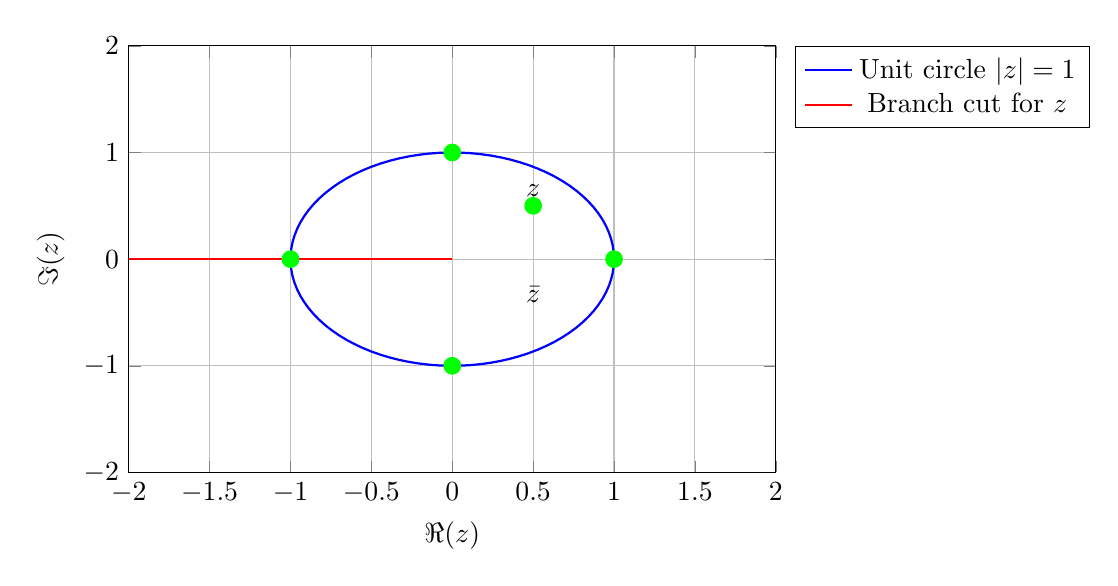
\begin{tikzpicture}
    \begin{axis}[
        width=9.8cm,
        height=7cm,
        xlabel={$\Re(z)$},
        ylabel={$\Im(z)$},
        xmin=-2, xmax=2,
        ymin=-2, ymax=2,
        grid=major,
        legend pos=outer north east
    ]
    
    % Draw the unit circle
    \addplot[blue, thick, samples=100, domain=0:360] ({cos(x)}, {sin(x)});
    \addlegendentry{Unit circle $|z| = 1$}
    
    % Draw the negative real axis (branch cut)
    \addplot[red, thick, samples=100, domain=-2:0] ({x}, {0});
    \addlegendentry{Branch cut for $\Log z$}
    
    % Mark some example points
    \addplot[only marks, mark=*, mark size=3pt, green] coordinates {
        (1, 0) (0, 1) (-1, 0) (0, -1) (0.5, 0.5)
    };
    
    % Add labels for complex conjugation
    \node[above] at (axis cs: 0.5, 0.5) {$z$};
    \node[above] at (axis cs: 0.5, -0.5) {$\bar{z}$};
    
    \end{axis}
\end{tikzpicture}
\caption{Problem 5.36: The complex plane showing important domains and regions. The unit circle represents $|z| = 1$, the red line shows the branch cut for $\Log z$ along the negative real axis, and the green points show example complex numbers including a point $z$ and its conjugate $\bar{z}$.}
\end{figure}

\begin{figure}[h]
\centering
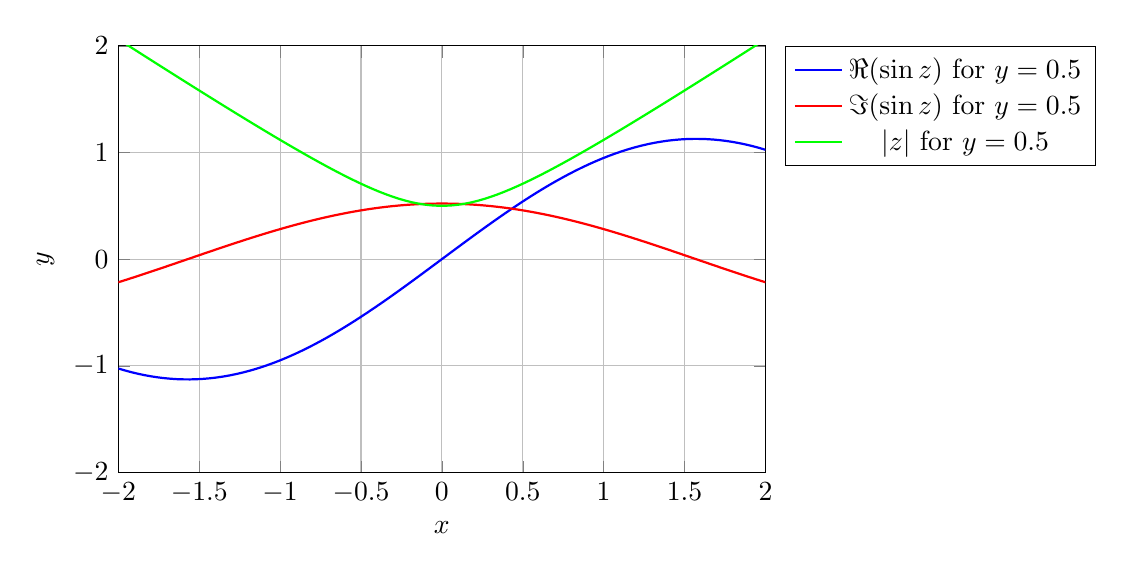
\begin{tikzpicture}
    \begin{axis}[
        width=9.8cm,
        height=7cm,
        xlabel={$x$},
        ylabel={$y$},
        xmin=-2, xmax=2,
        ymin=-2, ymax=2,
        grid=major,
        legend pos=outer north east
    ]
    
    % Plot the real part of sin(z) = sin(x)cosh(y)
    \addplot[blue, thick, samples=100, domain=-2:2] {sin(deg(x))*cosh(0.5)};
    \addlegendentry{$\Re(\sin z)$ for $y = 0.5$}
    
    % Plot the imaginary part of sin(z) = cos(x)sinh(y)
    \addplot[red, thick, samples=100, domain=-2:2] {cos(deg(x))*sinh(0.5)};
    \addlegendentry{$\Im(\sin z)$ for $y = 0.5$}
    
    % Plot |z| = sqrt(x^2 + y^2) for y = 0.5
    \addplot[green, thick, samples=100, domain=-2:2] {sqrt(x^2 + 0.25)};
    \addlegendentry{$|z|$ for $y = 0.5$}
    
    \end{axis}
\end{tikzpicture}
\caption{Problem 5.36: Real and imaginary parts of complex functions for fixed $y = 0.5$. The blue curve shows $\Re(\sin z) = \sin(x)\cosh(0.5)$, the red curve shows $\Im(\sin z) = \cos(x)\sinh(0.5)$, and the green curve shows $|z| = \sqrt{x^2 + 0.25}$.}
\end{figure}

\bigskip\noindent\textbf{Solution:}
i) Standard expansions give: $\sin z=\sin x\cosh y+i\cos x\sinh y$, $\cos z=\cos x\cosh y-i\sin x\sinh y$, $|z|=\sqrt{x^2+y^2}$, $\bar z=x-iy$, $\arg z=\arctan(y/x)$ ($z\ne 0$), $\Log z=\ln|z|+i\arg z$ ($z\ne 0$), $e^{z^2}=e^{x^2-y^2}(\cos 2xy+i\sin 2xy)$, $z^{\alpha}=e^{\alpha\Log z}$.\newline
ii) The Cauchy–Riemann equations hold on the stated sets: everywhere for (a),(b),(g); nowhere for (c),(d),(e); on $\mathbb{C}\setminus(-\infty,0]$ for branches of $\Log$ and $z^{\alpha}$, with the special cases as indicated.\newline
iii) Where differentiable: $(\sin z)'=\cos z$, $(\cos z)'=-\sin z$, $(\Log z)'=1/z$, $(e^{z^2})'=2z e^{z^2}$, $(z^{\alpha})'=\alpha z^{\alpha-1}$ (on the domain of the chosen branch).\qed


\begin{problembox}[5.37: Constant Function Condition]
Write \( f = u + iv \) and assume that \( f \) has a derivative at each point of an open disk \( D \) centered at (0, 0). If \( au^2 + bv^2 \) is constant on \( D \) for some real \( a \) and \( b \), not both 0, prove that \( f \) is constant on \( D \).
\end{problembox}

\noindent\textbf{Strategy:} Differentiate the equation \( au^2 + bv^2 = C \) and use the Cauchy-Riemann equations to obtain a system of linear equations. Show that the determinant of this system is non-zero, which implies that the partial derivatives vanish, making \( f \) constant.

\bigskip\noindent\textbf{Solution:}
Let $f=u+iv$ be complex differentiable on $D$ and suppose $au^2+bv^2\equiv C$ with $(a,b)\ne (0,0)$. Differentiate: $auu_x+bvv_x=0$ and $auu_y+bvv_y=0$. Using the Cauchy–Riemann equations $u_x=v_y$, $u_y=-v_x$, we obtain the linear system
\[\begin{pmatrix}au&bv\\ -bv&au\end{pmatrix}\begin{pmatrix}u_x\\ v_x\end{pmatrix}=\begin{pmatrix}0\\ 0\end{pmatrix}.\]
On $D$, the determinant is $a^2u^2+b^2v^2\ge 0$. If it is nonzero at a point, then $u_x=v_x=0$ there; by analyticity, $u_x\equiv v_x\equiv 0$ on the component, hence $u_y=v_y\equiv 0$ and $f$ is constant. If it vanishes at a point, then $u=v=0$ there; by the identity principle for holomorphic functions, $f\equiv 0$ in a neighborhood. In all cases $f$ is constant on $D$.

\section{Solving and Proving Techniques}

\subsection*{Proving Limits Exist}
\begin{itemize}
\item Use the definition of limit with $\varepsilon$-$\delta$ arguments
\item Apply the squeeze theorem when bounding functions
\item Use continuity of known functions (polynomials, exponentials, etc.)
\item Apply L'Hôpital's rule for indeterminate forms
\item Use Taylor series expansions for complex functions
\item Apply the Cauchy criterion for sequences
\end{itemize}

\subsection*{Proving Differentiability}
\begin{itemize}
\item Use the definition of derivative and show the limit exists
\item Apply known differentiation rules (sum, product, quotient, chain)
\item Use the fact that differentiability implies continuity
\item Apply the Mean Value Theorem to relate difference quotients
\item Use component-wise differentiation for vector-valued functions
\item Apply the Cauchy-Riemann equations for complex functions
\end{itemize}

\subsection*{Using the Mean Value Theorem}
\begin{itemize}
\item Express difference quotients in terms of derivatives at intermediate points
\item Prove existence of points where derivatives take specific values
\item Establish bounds on function values using derivative bounds
\item Prove monotonicity by analyzing derivative signs
\item Show convergence of sequences using derivative bounds
\item Prove fixed point theorems using contraction properties
\end{itemize}

\subsection*{Proving Existence of Points}
\begin{itemize}
\item Apply Rolle's Theorem when function values are equal at endpoints
\item Use the Intermediate Value Theorem for continuous functions
\item Apply the Mean Value Theorem to find intermediate points
\item Use the Extreme Value Theorem on closed, bounded intervals
\item Apply the Bolzano-Weierstrass theorem for sequences
\item Use the contraction mapping theorem for fixed points
\end{itemize}

\subsection*{Working with Derivatives}
\begin{itemize}
\item Use logarithmic differentiation for products and quotients
\item Apply Leibniz's formula for higher derivatives of products
\item Use mathematical induction for derivative formulas
\item Apply the chain rule for composite functions
\item Use the product rule for dot products of vector functions
\item Apply the quotient rule and simplify using algebra
\end{itemize}

\subsection*{Proving Inequalities}
\begin{itemize}
\item Use the Mean Value Theorem to bound differences
\item Apply the triangle inequality for vector functions
\item Use the fact that derivatives bound function growth
\item Apply the Cauchy-Schwarz inequality when appropriate
\item Use the fact that increasing functions preserve inequalities
\item Apply the squeeze theorem for limit comparisons
\end{itemize}

\subsection*{Working with Complex Functions}
\begin{itemize}
\item Separate real and imaginary parts using standard expansions
\item Apply the Cauchy-Riemann equations to check differentiability
\item Use the fact that complex conjugation is continuous and linear
\item Apply the identity principle for holomorphic functions
\item Use the fact that constant norm implies orthogonality with derivative
\item Apply standard complex differentiation rules
\end{itemize}

\subsection*{Proving Uniqueness}
\begin{itemize}
\item Use the fact that differentiable functions are continuous
\item Apply the identity principle for holomorphic functions
\item Use the fact that constant functions have zero derivatives
\item Apply the contraction mapping theorem for fixed points
\item Use the fact that linear independence implies non-zero Wronskian
\item Apply the fact that analytic functions are determined by their values on sets with limit points
\end{itemize}

\subsection*{Using Proof by Contradiction}
\begin{itemize}
\item Assume the opposite of what you want to prove
\item Use the Mean Value Theorem to derive contradictions
\item Apply the fact that limits must be unique
\item Use the fact that continuous functions preserve connectedness
\item Apply the fact that differentiable functions are continuous
\item Use the fact that bounded sequences have convergent subsequences
\end{itemize}

\subsection*{Working with Sequences and Series}
\begin{itemize}
\item Use the Cauchy criterion to prove convergence
\item Apply the Mean Value Theorem to bound sequence differences
\item Use the fact that bounded monotone sequences converge
\item Apply the squeeze theorem for sequence limits
\item Use the fact that convergent sequences are bounded
\item Apply the fact that subsequences of convergent sequences converge to the same limit
\end{itemize}

\subsection*{Proving Continuity}
\begin{itemize}
\item Use the definition of continuity with $\varepsilon$-$\delta$ arguments
\item Apply the fact that differentiable functions are continuous
\item Use the fact that sums, products, and compositions of continuous functions are continuous
\item Apply the fact that uniform limits of continuous functions are continuous
\item Use the fact that inverse functions of strictly monotone continuous functions are continuous
\item Apply the fact that vector-valued functions are continuous if and only if each component is continuous
\end{itemize}

